% flashcards-title: Structure diagram of a two-step calculation
% flashcards-desc: The numbers 7 and 2 each have an arrow into a box marked with a subtraction sign. An arrow leaves that box and meets an arrow from the number 3 at a box marked with a multiplication sign. An arrow leaves the multiplication box and ends at a box holding a question mark. No written expression and no result value are shown.
\documentclass[tikz]{standalone}
\usetikzlibrary{arrows.meta,patterns}

\definecolor{qraNavy}{HTML}{17324D}
\definecolor{qraBlue}{HTML}{2B6CB0}
\definecolor{qraGold}{HTML}{B7791F}
\definecolor{qraPale}{HTML}{EAF2F8}
\definecolor{qraGray}{HTML}{5C6773}

\tikzset{
  qra axis/.style={draw=qraNavy, line width=1.2pt},
  qra tick/.style={draw=qraNavy, line width=1pt},
  qra guide/.style={draw=qraGray, densely dashed, line width=0.8pt},
  qra counter/.style={circle, draw=qraNavy, fill=qraPale, line width=0.9pt, minimum size=7mm, inner sep=0pt},
  qra label/.style={font=\sffamily\bfseries, text=qraNavy},
  qra small label/.style={font=\sffamily, text=qraNavy},
}

\begin{document}
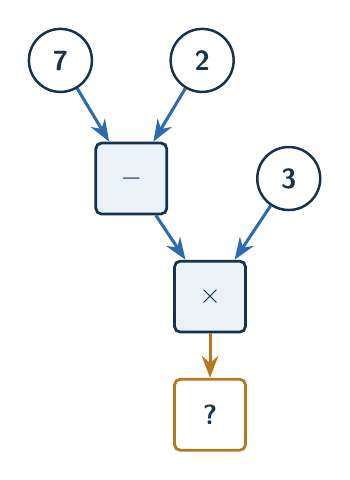
\begin{tikzpicture}[
  value/.style={qra label, circle, draw=qraNavy, fill=white,
    line width=0.9pt, minimum size=8mm, inner sep=1pt},
  op/.style={qra label, rectangle, rounded corners=2pt, draw=qraNavy,
    fill=qraPale, line width=1pt, minimum size=9mm, inner sep=2pt},
  flow/.style={draw=qraBlue, line width=1.1pt, -{Stealth[length=2.8mm]}}
]
  \node[value] (n7) at (0,0) {7};
  \node[value] (n2) at (1.8,0) {2};
  \node[op] (minus) at (0.9,-1.5) {$-$};
  \node[value] (n3) at (2.9,-1.5) {3};
  \node[op] (times) at (1.9,-3.0) {$\times$};
  \node[op, fill=white, draw=qraGold] (result) at (1.9,-4.5) {?};

  \draw[flow] (n7) -- (minus);
  \draw[flow] (n2) -- (minus);
  \draw[flow] (minus) -- (times);
  \draw[flow] (n3) -- (times);
  \draw[flow, draw=qraGold] (times) -- (result);
\end{tikzpicture}
\end{document}
